\chapter{Background}\label{chp:background}


\section{Passwords}
Passwords are the common way of authenticating users upon access to sites on the Internet. The idea is that only the user and the target service know the password, and the user has to provide the correct password before access is granted. Passwords are a much discussed theme and claiming that passwords are not always used in the correct manner is not an overreaction. The main problem seems to be that good passwords and the human memory does not go well together~\cite{memorability_yan}. For passwords to be sufficient as authentication each user has to be forced into using long complex password, or even use one generated for them, with the problem being that it is easily forgotten. Furthermore, if a user was able to memorize \emph{one} "good" password, he will probably use this for all of his accounts, so that if one of the services is compromised and user information leaked, all his accounts may be compromised. With all of this in mind it is easy to say that everybody should use complex, unique passwords for each account, but in practice this is not feasible. Florêncio and Herley ~\cite{password-habits} conducted a large scale study of passwords habits in 2007, revealing that a user on average has 25 different accounts protected by passwords. On average these sites are protected by about 7 distinct password, where 5 of them are rapidly re-used.
\par Password authentication requires the authenticating server to store something related to the password, if this is stolen the password will in most cases be compromised as well, even if the server did not store the clear text password. Attackers will, in most cases, be able to retrieve the password eventually. After obtaining the username and password for one service the attacker would try this user data on other services and compromise these as well. 
\par If a user was to have different passwords for each site, these might still easily be compromised. Ives et al. ~\cite{domino-effect} discuss this "domino effect", where intrusion to one domain can compromise several others, if users have re-used passwords.  A normal user will typically try to log in by trial-and-error ~\cite{single-pw-auth}, if the first password does not work, the user will try with another of his passwords. This way passwords might be lost through phishing attacks where a user is tricked into trying to log in to a fake site. It is thus clear that some kind of system is needed to allow a human user to manage strong passwords. The best case would be if each user, for each of his 25 accounts had a unique password of satisfying strength, this is of course not possible.

\subsection{Password strength}\label{password-strength}
How to measure the strength of passwords is a well known and discussed problem, but the naive approach says that password strength is related to how strong a password is against brute force attacks \cite{password-strength}. Length and complexity are the most thought of parameters to measure such strength. A perfect password would thus be one as long as allowed by the system consisting of random characters from all possible characters, this one would also be changed frequently. All these characteristics challenge how the human brain works. In addition to the objective strength of the password, techniques making it harder for a computer to repeatedly try different passwords may be applied. Such techniques include CAPTACHAS \cite{captcha} which are puzzles supposed to require a human to be able to solve, thus making brute force using a computer harder. Or techniques making it easier for the user to remember multiple strong passwords.
\par Yan et al.~\cite{memorability_yan} investigate the trade-off between security of passwords versus memorability allowing humans to remember them. An important regarding this trade-off is that most sites applying advice and policies on how to create strong passwords, do not take into account if the recommended passwords are hard or easy to remember. There is no point in having a strong password if the user is going to forget it. Yan et al. suggest that passwords should appear random but be constructed using a  mnemonic structure such ass passphrases. The idea here is to generate a random looking password by memorizing a familiar sentence and using the first letters of each word as the password. 
\par Florêncio et al.~\cite{strong-pws_florencio} investigate another matter; do strong passwords accomplish anything? The point is that no matter how long and complex password users chose they are still subject to the most dangerous and common threats (phishing, keylogging or access attacks). Especially access attacks, which includes shoulder surfing and direct access to a machine where a autofilling password manager is used, are unaffected by the strength of the password.  The reason for enforcing strong passwords seems to be to protect against bulk guessing attacks, against other attacks, typically offline attacks, shorter passwords is usually sufficient. Offline attacks depends mainly on the strength of the hash function used.

\par Some services my require their users to include characters from different groups, such as digits, symbols and upper case letters, and possibly a minimum length. Table \ref{pw-strength} illustrates the effects of password length and character set. The values represents the possible values a key might have given the length and character set. E.g. using only digits and length 4 gives $10^4$ possible combinations. The bigger the key space is the harder it is to perform a brute force attack. Note that the key space increase more rapidly with increased password length, than by increasing complexity of the characters used. If the character set is increased from 10 to 95 the key space increase 800 times given length of 4 characters, while increasing the length from 4 to 16 increase the key space one billion times with a character set of 10. Even if both character set and password length contribute to the strength of a password, length is the dominant factor.


\definecolor{Gray}{gray}{0.9}

\begin{figure}
    \centering
    \begin{tabular}{c|c|c|c|c|c|}
    \multicolumn{6}{c}{Password length}\\\cline{2-6}
    \multirow{6}{*}{\begin{sideways}Character set\end{sideways}}
      &\cellcolor{Gray}&\cellcolor{Gray}4&\cellcolor{Gray}8&\cellcolor{Gray}12&\cellcolor{Gray}16\\\cline{2-6}
    &\cellcolor{Gray}10&$10^4$&$10^8$&$10^{12}$&$10^{16}$\\\cline{2-6}
    &\cellcolor{Gray}26&$5\cdot10^5$&$2\cdot10^{11}$&$10^{17}$&$4\cdot10^{22}$\\\cline{2-6}
    &\cellcolor{Gray}36&$2\cdot 10^6$&$3\cdot10^{12}$&$5\cdot10^{18}$&$8\cdot10^{24}$\\\cline{2-6}
    &\cellcolor{Gray}62&$10^7$&$2\cdot10^{14}$&$3\cdot10^{21}$&$5\cdot10^{28}$\\\cline{2-6}
    &\cellcolor{Gray}95&$8\cdot10^7$&$7\cdot10^{15}$&$5\cdot10^{23}$&$4\cdot10^{31}$\\\cline{2-6}
    \end{tabular}
    \caption{\cite{nist-guide} Table showing the possible keyspace of passwords, given length and character set. }
    \label{pw-strength}

\end{figure}


\par The main point to take from this is that no matter how strong password a user may chose, it is still vulnerable to attacks. It is thus most important to limit the consequences from a possible password breach, by never re-using passwords on several accounts. This way, if an attacker manage to steal a password all other accounts of the same user is still safe. 

\paragraph{Password strength meters} are a common way used by many sites on the Internet to aid their users when selecting passwords. Common meters use colored progression bars together with a word or short comment stating if the entered password is evaluated as "bad", "poor" or "strong". Ur et al. \cite{password-meters2} found that password meters actually lead users into choosing longer and stronger passwords, but they also argue that enforcing such policies might frustrate users and possibly lead them into writing passwords down, use weak password management schemes or re-use the same password across many sites. The most common requirements used by passwords meters of known web services can be summarized as the following \cite{password-meters}:
\begin{itemize}
    \item{Length and character selection} are part of most password meters. It is normal to disallow passwords shorter, and sometimes longer, than a given range, which may vary. A variation of different characters can be required, namely different kinds of symbols or capital letters. Spaces may be allowed in between other characters, at the start or end of the password, or not at all. Some sites checks for sequences of the same character as well.
    \item{Personal information.} Information registered by the user are evaluated by some meters, typically name, email and date of birth are checked against in original and transformed forms. This means that a password like "4nD3r?1991" ("anders1991" transformed) which look strong, will be evaluated as weak.
    \item{Dictionary checks.} Make sure that the password does not include any dictionary words by matching it with a dictionary of common words. 
\end{itemize}

%\paragraph{Entropy}
%\todo{write about entropy, \cite{password-policy, shannon-entropy}}
%Entropy, as specified by Shannon~\cite{shannon-entropy} in 1948, is defined as the average information in each sample. Entropy, and variations of it, is frequently used as a measure of password quality. 
%

\par The conclusion on what "good" passwords are, is not clear, but the one thing agreed upon seems to be that re-use of passwords are the biggest threat. It is a fact that the human brain is not capable of remembering different passwords for each account on the Internet, thus the need for an aiding application such as the one discussed in this project. If a user is able to at least have different passwords for each account, the consequences of a password breach is severely limited. The loss of one account will not compromise any other accounts. 

\subsection{Password Storage}\label{pw-storage}
Internet services using password as authentication method typically have to store information about their users, associating a user and a password. How this information is kept secure can not be controlled by the user, but it important for passwords to work. Especially since many users tend to re-use their passwords on several account~\cite{domino-effect}, thus if one account is compromised, many others might also be lost. It is a fact that these kinds of breaches do happen from time to time, and attackers might even post the credentials online\footnote{Hackers post millions of stolen Gmail passwords - \url{http://www.cbsnews.com/news/russian-hackers-steal-5-million-gmail-passwords/} } If the service stores the passwords in plain text, leakage might directly lose passwords if the database gets lost.
\par Most online accounts try to make it harder for attackers to compromise the accounts of their users. The most used technique are hashing of the passwords before storing them, making it hard for an attacker to recover the actual passwords even if the database is broken. Hashing means applying a one-way function on the plain text password, producing a fixed length hash value which is stored instead of the plain text. When a user wants to log in the password is sent to the server where it is hashed again using the same one-way function and then compared to the stored hash value. If the database where these hashes are stored is compromised, making the hashes available to the attacker, he can no longer directly use the data to steal account. The attacker would have to first perform an offline attack, cracking (see \autoref{atck}) the hashes to recover the plain text passwords, which requires a lot of effort and time to carry out. 
\par The problem with only hashing the passwords is that the hash of a given password will be the same every time, making it possible to recognize known password hashes through the use of big table containing the hashes of known passwords. This way a hash might get cracked quite easily . To circumvent this problem a service might add a random \emph{salt} to the password before hashing it. This way the hash of a user's password will be unique even for users with the same password. A salt is a randomly generated nonce, which is concatenated with the password before hashing, and then stored alongside the hash value in the user database. To authenticate a user the server concatenates the entered password with the salt from 

\begin{example}
Let the following be the records of a user database, and $H$ a cryptographically strong hash function.
    \begin{table}[ht!]
        \centering
    \begin{tabular}{|c|c|c|}
        \hline
        Username & Hash & Salt \\
        \hline
        Bob & 3aaF4A4PxZ & wRaE3Z9oa6 \\
        \hline
        $\dots$ & $\dots$ & $\dots$ \\
        \hline
    \end{tabular}
    \end{table}
\par To authenticate, Bob would enter his password, $pwd=\text{ letno1in }$, which is sent to the server. The server then concatenate $pwd$ with the salt from Bob's entry in the database, and then apply the hash function to the result. If this is the same as the stored hash, Bob is authenticated.\\
 \centerline{\text{ If }   $H(letno1inwRaE3Z9oa6) = 3aaF4A4PxZ \rightarrow \text{Bob authenticated}.$  }

\end{example}



The hash function can be made even stronger by using a keyed hash function~\cite{keyedhash} or simply encrypting the hashes, requiring a shared secret key between the user and the server. As a user one can not control how different services store passwords, which is another important argument for never re-using passwords. Even if most sites store passwords securely, one badly configured site might compromise all the others. 



\subsection{Attacks}\label{atck}
Passwords are often the only barrier stopping adversaries from directly accessing the accounts of a user. The combination of user name and password are the easiest point of attack, and thus the most valuable to break. There are several methods used to attack password authentication, trying to retrieve passwords. The most important attacks~\cite{nist-guide, strong-pws_florencio}, including access attacks and offline/online attacks, is discussed in the following section. 
\paragraph{Capturing} of passwords directly from the server responsible for the authentication involves the attacker acquiring password data through breaking into the data storage, eavesdropping on communication channels or through monitoring the user by other means. The first, most basic threat is to simply steal the stored password from an insecure server, this would require a weak configured server storing the passwords in plain text. This is mitigated by storing only cryptographic hashes of passwords, which allows the server to authenticate users while preventing attackers from determining the actual passwords without \emph{cracking} the hashes. Capturing can also be done through direct access attacks~\cite{guide-pws} such as shoulder surfing or console access on computer with autofilling password managers or "remember be"-functions.

\paragraph{Online attacks} are attacks directed towards the server's public user interface. Such attacks can be mounted simply by guessing username/password-pairs and sending authentication requests to the server, usually automated by scripts. The approach when carrying out such attacks are either by doing breadth-first or depth-first. The former involves trying one password one all accounts first before trying a new password. This technique would generate unusually high data load which would trigger alarms on the server. Depth-first involves trying a lot of different password already knowing the username to attack. This would usually be blocked by lockout policies limiting the number of attempt allowed in a given interval.

\paragraph{Offline attacks} are directed towards the backend of sites. To carry out such an attack, one would have to first access the system gaining access to the password file without being detected. If detected while gaining access to the passwords, an system administrator might be able to force password resets by all the users, greatly limiting the time an attacker has to \emph{crack} the passwords in the file.

\paragraph{Cracking} requires the attacker to go through several steps. First acquiring the hash of a user account or a whole file of hashes for a site. Next, one would try to find a sequence of strings yielding the same hash as the actual password. Cracking if much harder if the server uses salts to randomize the hashes.
\par \emph{ Rainbow tables }~\cite{rainbow-tables} is a technique employed by attackers to speed up this process. Rainbow tables are precomputed table of hashes, allows the attacker to compute a set of hashes once and use these values several times, thus providing a space-time trade-off. This involves using more space, since all the computed hash values would have to be stored somewhere, but allowing a much shorter computation time to brute-force a hash. The technique stores chains of hashes as shown in figure ~\ref{rainbow-table}, storing only the first and last value of the chain. The attacker then searches for a given hash in the set of end points, if no match is found the hash function is applied and a new search conducted. This process continues, until a match is found, the plain text is then computed from the start value of the chain, applying the hash function the same amount of times it took to find a match in the chain. 

\begin{figure}[ht]
    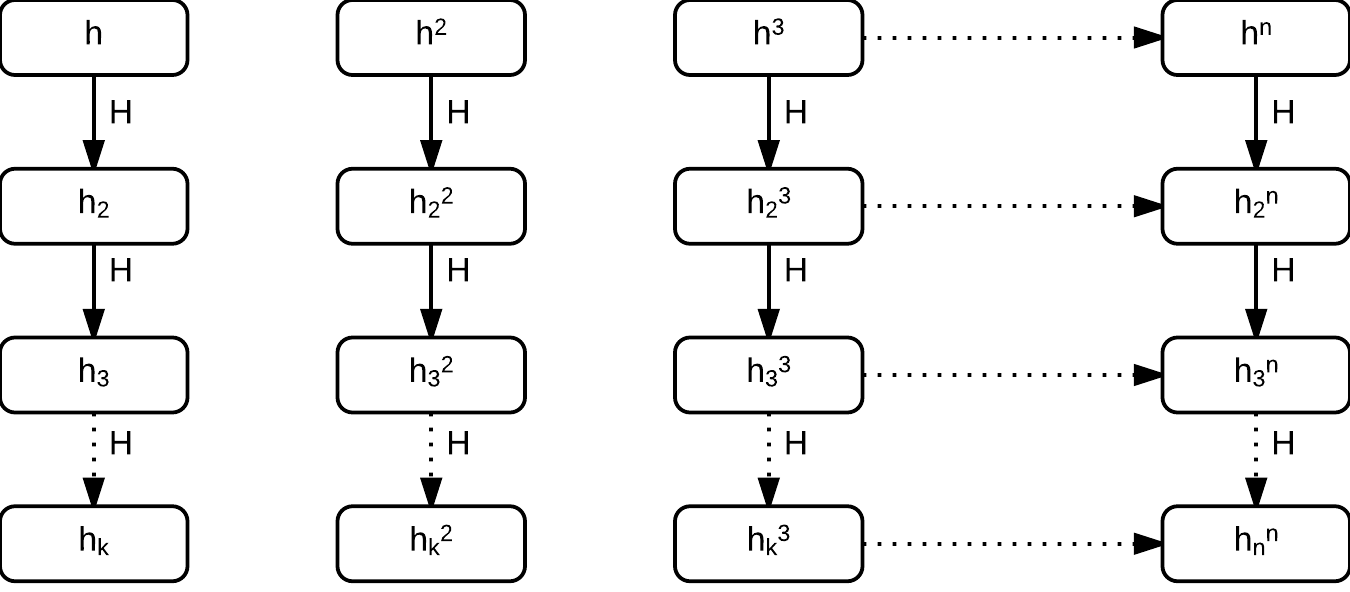
\includegraphics[width=\textwidth]{rainbow-table}
    \caption{Rainbow table}
    \label{rainbow-table}
\end{figure}


\subsection{Offline-online Gap and Classifying of Accounts.}\label{classification} Florêncio et al.~\cite{guide-pws} shows that a password have to be able to withstand at least $10^6$ guesses to be safe against online attacks. To survive offline attacks at least $10^{14}$ would be necessary. The point highlighted is that a password able to withstand $10^{10}$ guesses, is no more likely to survive a offline attack than a password only protected against $10^6$ guesses. 
\par Florêncio et al. thus suggest that users should classify all accounts into categories ranging from "Don't-care" to "Ultra-sensitive". The idea is that it is no point in using complex and long password on an account which doesn't contain any sensitive information. For critical accounts related to finance, primary employment or other highly confidential documents would typically use multiple factors of authentication~\cite{2-factor-auth}. Accounts such as social media would probably be categorized as "medium-consequence" as loss of such accounts would be more about time and effort, than financial loss. It is of course up to the user to categorize how critical it would be to lose each account (see ~\cite{guide-pws} for an example category division). 
\par The important point is that accounts should be treated differently, there is no point in using a 20 characters long password on an online chess game account, while it would be reasonable on a online banking account. This can be utilized to make password management more adaptable and easy to use. Especially when using a password management scheme as the one evaluated in this project, it is very beneficial to lower the average length of password, while still having long passwords for the important accounts.

%\section{The User}\label{sec:the-user}
%"Good passwords" as discussed in \ref{password-strength} does not go well with the human memory. The first limitation which will be an important property later are the limitation to how much data we can store in immediate memory, this limit was showed to be 7 chunks of data at once~\cite{magic-seven_miller}. This data can not be from a random selection which is what a good password requires.   


\section{Password Management}
As seen in the previous sections passwords introduce a dilemma as passwords are supposed to be hard to "guess" and thus hard to remember. The naive solution to this problem is to either use one password for many accounts or to write down passwords. To make the process of managing passwords easier several techniques and tools have been suggested~\cite{management-strategies}. Examples are reminder features including the "I forgot me password"-function most websites implement, browser cookies allowing the user to stay logged in across browser sessions or services storing the password. These are all "computer aided" tools, which will store or keep the user logged in without actually having to remember the password. This usually limits the user to stay on the same machine while using the account, this way the user will probably forget the password and be forced into using the "forgot my password"-function eventually. A different approach is to use a technique to actually remember the passwords without storing them.
\par Consider a password management scheme to be a method helping the user remember password without actually storing them. The term password management software or password mangers are used about solutions which store the passwords in some way.

\subsection{Password management schemes}
 
Password creation and memorization techniques assists the user in remembering passwords, trying to circumvent the limitations of the human memory~\cite{human-memory}. 
\par Blocki et al. \cite{naturally-rehearsing} consider 4 different examples of password managements schemes to illustrate how users might choose and remember their passwords.
\begin{itemize}
    \item{ Reuse Weak. } When a user selects a random phrase or word $w$ and reuse this as the password $p_i=w$ for all accounts. While maybe not very strong, this is the most simple example of a password management scheme.
    \item{ Reuse Strong. } Same as reuse weak but the user chose four random words $w_1,w_2,w_3,w_4$ and reuse the concatenation of these as the password $p_i = w_1w_2w_3w_4$ for all his accounts.
    \item{Lifehacker.} User choses three random words $w_1, w_2, w_3$ as a base password $b=w_1w_2w_3$ as well as a derivation rule $d$ used to derive unique data from the site names for each password \footnote{How to Update Your Insecure Passwords and Make Them Easy to Use.\url{http://lifehacker.com/5631203/how-to-update-your-insecure-passwords-and-make-them-easy-to-use}}. Example of a derivation rule could be the first and last three letters of the service name. The password for account $A_i$ would then be $p_i = b d(A_i)$ with $d(A_i)$ being the string derived from the site name. In practice a password generated using the method might look like "facthreerandomwordsook". 
    \item{Strong Random and Independent.} User choses new words $w^i_1, w^i_2, w^i_3, w^i_4$ for each account to be used as passwords $p_i = w^i_1w^i_2w^i_3w^i_4$.
\end{itemize}
It is clear that the three former schemes are much easier to use than the last one. Most user would prefer the first ones because they does not require much if any rehearsal while the one strong scheme would require too much effort in terms of rehearsing and memorization. This trade-off between usability and security is the main problem when designing password management schemes. For a scheme to be popular it cannot require too much extra rehearsal, while a secure scheme most of the time will require some.



\subsection{Password manager software.} \label{subsec:pms}
Applications meant to keep passwords safe for the user. These applications can either be stand alone programs or, more common, browser extensions such as LastPass \footnote{LastPass \url{https://lastpass.com/}}. LastPass provides an user interface to generate and store passwords for online services, as well as form fillers to enter them when logging in. The passwords are encrypted using a master password protecting the user credentials against both server leakage and insiders accessing the data. Such systems usually provides a lot of extra features such as automatically changing of passwords and syncing between devices. 

\paragraph{Built-in browser password managers.} Most modern browsers provide "remember password" functions. These functions act similar to software like LastPass, by storing the users passwords in some fashion, then reproduce it when login in. 

These kinds of systems and applications requires the user to trust that the implemented systems are secure enough to prevent adversaries, both insiders and outsiders, stealing credentials stored by the services. Software aiding the user by storing passwords often also provide autofill-functions, automatically filling in the username and password of the associated site. Silver et al. \cite{pw-managment-attacks} propose attacks exploiting these autofill functions to extract passwords from the password manager, the most basic example attack is shown in example \ref{rouge-wifi}. Despite of the obvious weaknesses in many password managers, they still argue that password managers can strengthen credential security if implemented correctly.  
\begin{example}\label{rouge-wifi}
    Consider a user connecting to a open wifi at a coffee bar or another public place. It is not unusual to present the user with a "landing page" asking for approval of some usage agreement. The rouge wifi provider could include multiple iframes\footnote{\url{http://www.w3schools.com/tags/tag_iframe.asp}} pointing to the login pages of common sites the user probably have stored credentials for. See \autoref{rouge-wifi-page}. By injecting javascript in the iframes the attacker can extract all the usernames and passwords autofilled by the password manager. Note that the iframes displayed in the figure are not visible to the user, to him it looks like a standard landing/welcome page. Silver et al. \cite{pw-managment-attacks} claim that six out of ten password managers were vulnerable to this simple attack.


\begin{figure}
    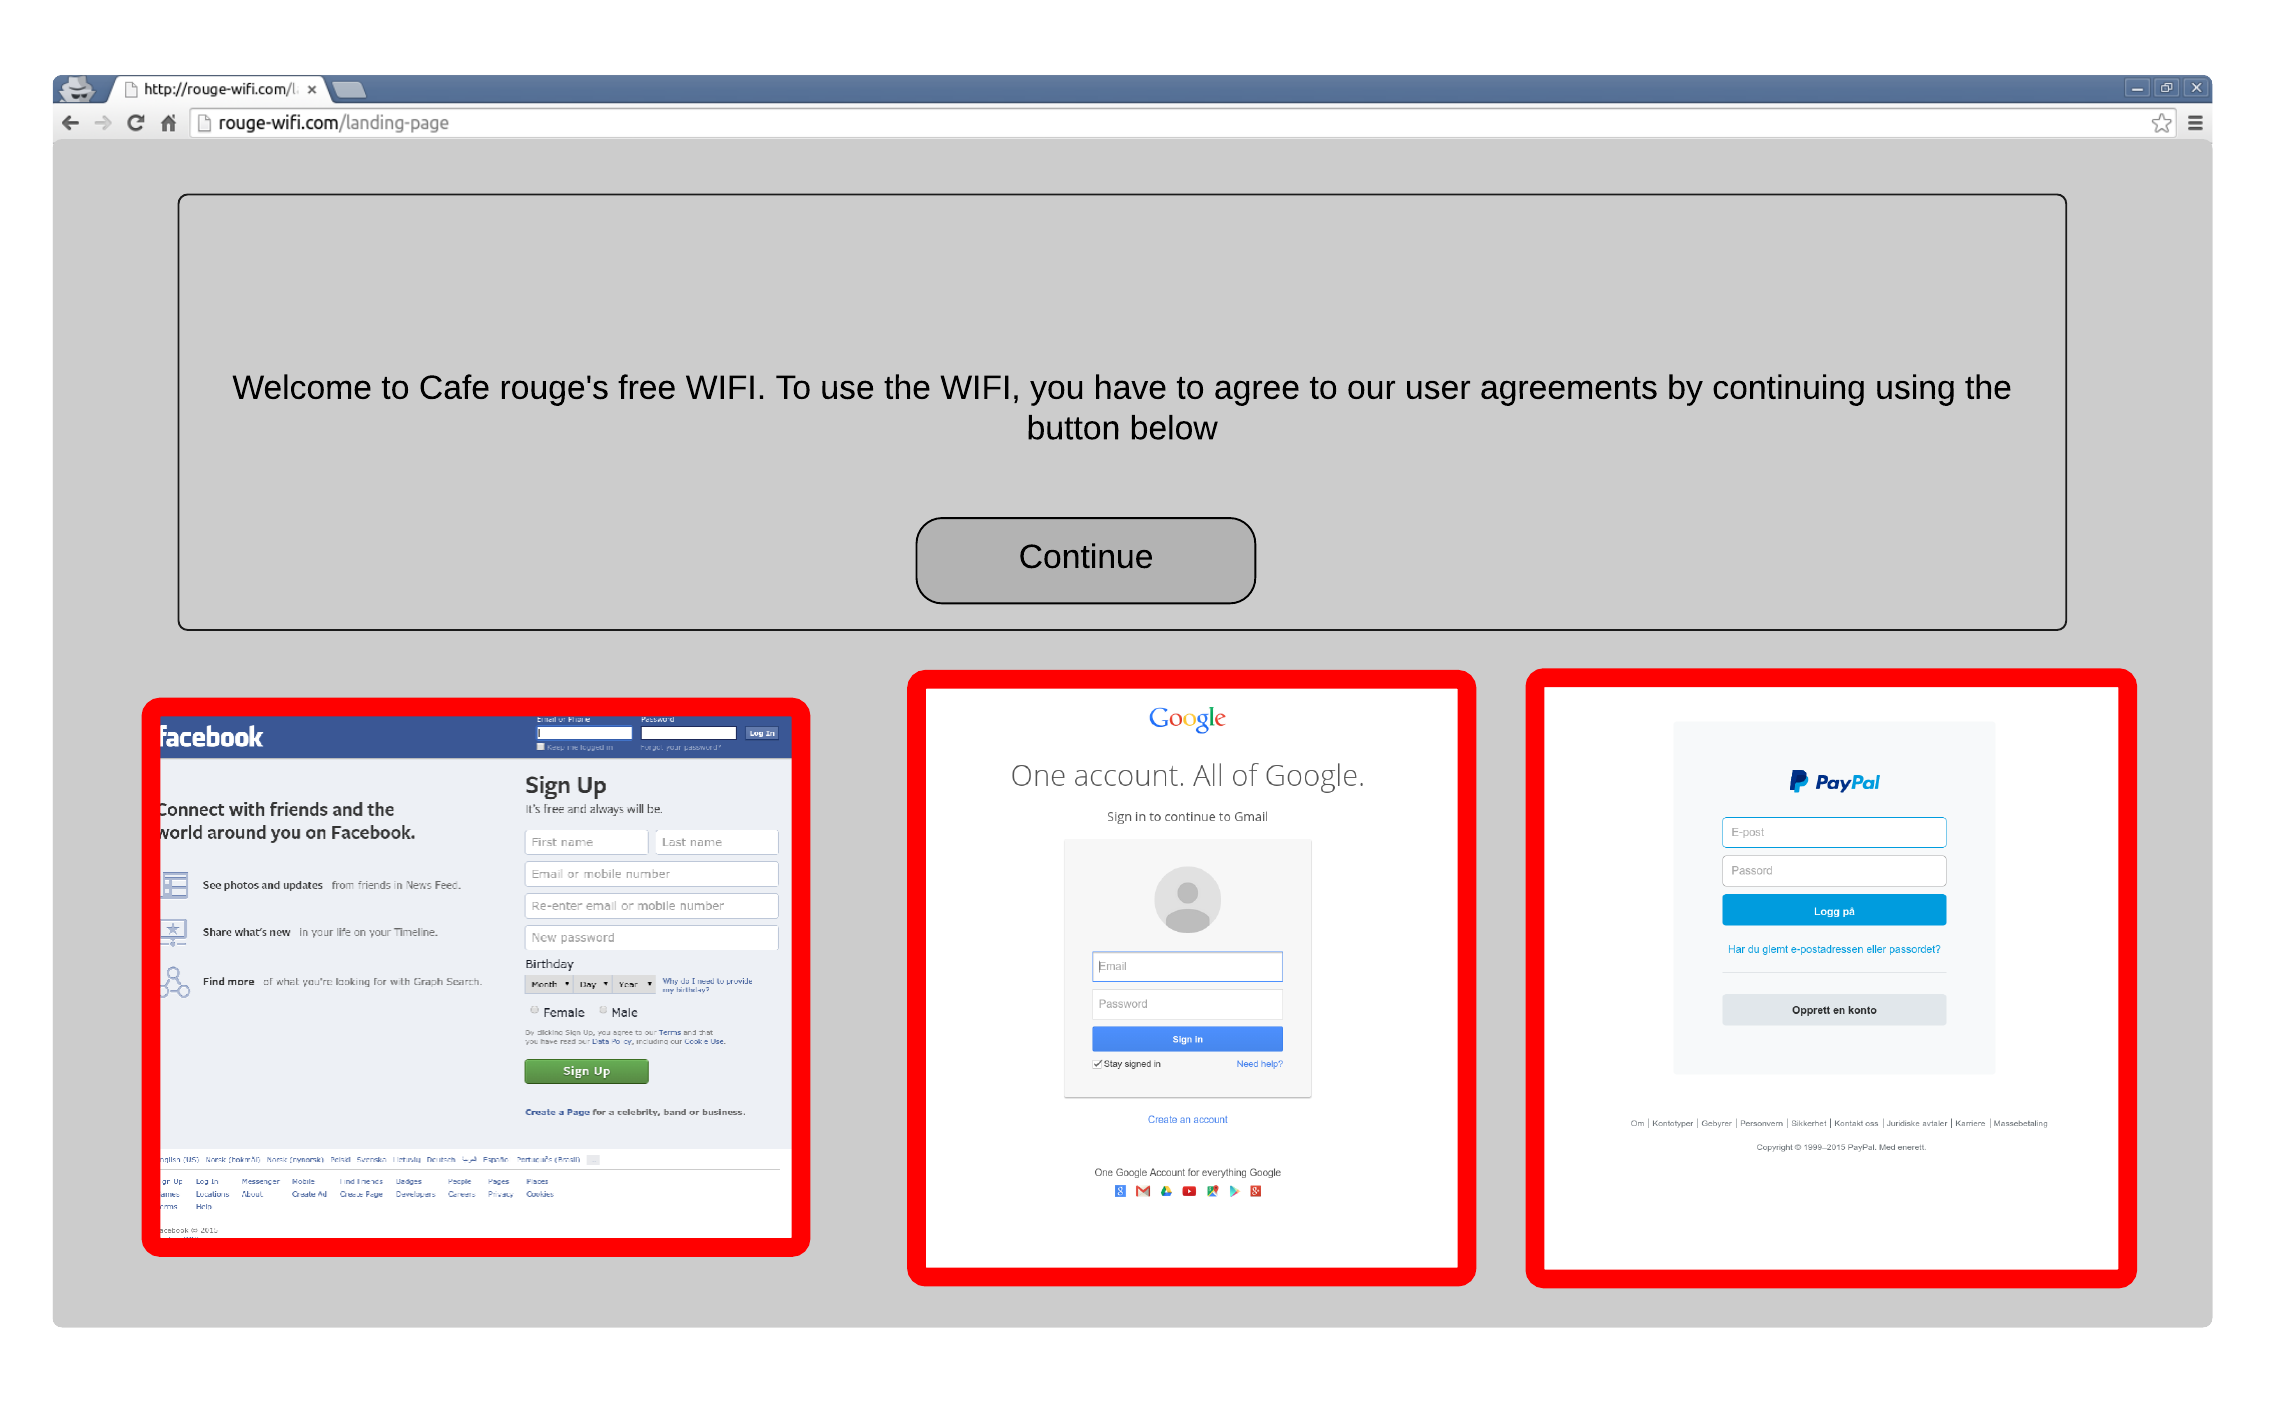
\includegraphics[width=\textwidth]{rouge-wifi-page}
    \caption{Rouge wifi landing page containing iframes with common sites, used to steal password form a autofilling password manager.} 
    \label{rouge-wifi-page}
\end{figure}

\end{example}

\par Even if the password manager is secure against autofill-attacks, or if it does not include the feature, the manager might still be at risk. If the account storing all the usernames and passwords of a user where to be compromised, all the sites would be compromised, so it is important that the password manager is even more secure than the sites themselves. Zhao et al. \cite{lastpass-security} identified several vulnerabilities in the LastPass implementation, even though no known breaches has been reported. They investigate different types of attacks, including attacks on local decrypted credentials; request monitoring attacks which tries to intercept request between the password manager and related cloud-storage; as well as brute-force attacks trying to crack the master password. The conclusion is that password managers are double-edged swords, in theory they help make password authentication stronger, but if implemented slightly wrong may be a major vulnerability. Storing all the passwords at one place makes a obvious point of attack for adversaries since breaking the managers most of the time would break all accounts stored within.



\section{Usability Model}\label{sec:usability-model}
This section presents the usability model defined by Blocki et al. \cite{naturally-rehearsing}, which predicts the effort required of a user to keep a set of secrets memorized without forgetting it. It will be presented in the context of password management schemes, in particular the human computable password management scheme relied on in this project. The model will later be used to analyze the usability of the scheme and related applications.

\subsection{Definitions}
A password management scheme generates and keeps track of passwords $p_1, \dots, p_m \in P$ for all $m \in A$ accounts of a user. $P$ is all possible passwords. Let $(\hat c, \hat a)$ represent an association between an object (e.g. letter or picture) and a related  mapping (typically a digit between 1 and 10). A user have to rehearse the association $(\hat c, \hat a)$ to avoid forgetting it. Next two schedules are defined defining how often a user has to rehearse to not forget a association, and how often he visits an account.

\begin{definition}\label{rehearsal-schedule}
    \cite{hcp-blocki} A rehearsal schedule for an object-mapping association $(\hat c, \hat a)$ is a series of points in time $t^{\hat c}_0 < t^{\hat c}_1 < \dots$. A rehearsal requirement for each $i \ge 0$ says that the object-mapping association pair must be rehearsed at least once in the time interval $[ t^{\hat c}_i, t^{\hat c}_i+1) = \{x \in \mathbb{R} \vert t^{\hat c}_i \le x < t^{\hat c}_{i+1} \} $.
\end{definition}
A rehearsal schedule as defined in definition \ref{rehearsal-schedule} is said to be sufficient if a user can keep an association in his memory without forgetting it by following the schedule.

\paragraph{Visitation schedule \cite{hcp-blocki}} is a series of numbers $\tau^i_0 < \tau^i_1 < ...$ representing the points in time when a user visits account $A_i$. This schedule cannot be known exactly so it is modeled using a random process with a parameter $\lambda_i$ based on the average time between visits to account $A_i$ - $E[\tau^i_{j+1} - \tau^i_j]$.
\par A rehearsal requirement can also be satisfied naturally if a user visits an account using the object $\hat c$ during the interval $[ t^{\hat c}_i, t^{\hat c}_i+1)$, as defined in definition \ref{natural-rehearsal},

\begin{definition}\label{natural-rehearsal}\cite{hcp-blocki}
     A rehearsal requirement $[ t^{\hat c}_i, t^{\hat c}_i+1)$ is naturally satisfied by a visitation schedule $\tau^i_0 < \tau^i_1 <\dots$ if for any $j \in [m]$ and $k \in \mathbb{N}$ so that $\hat c \in c_j$ and $\tau^j_ki \in [ t^{\hat c}_i, t^{\hat c}_i+1)$. Let \\
    \begin{large}
    \centerline{ $ER_{t,\hat c} = \vert\{ i \vert t^{\hat c}_{i+1} \le t \wedge \forall j ,k.(\hat c \notin c_j \wedge \tau^j_k \notin [t^{\hat c}_i, t^{\hat c}_i))\} \vert$ }
    \end{large}
    denote how many extra rehearsals required, that are \emph{not} satisfied by the visitation schedule, during time time interval $[0,t]$
\end{definition}




\subsection{Model}
The core of the model is that usability depends on rehearsal required to remember all passwords, relative to the visitation schedule of the specific user. How hard it is for any given user to remember a relation between object may vary from person to person depending on mnemonic technique and genetic conditions. This is adjusted for in the model by the constant $s$ representing the combined strength of mnemonic technique and the memory of a user. Next, consider two different rehearsal requirements specifying what is needed to maintain a memory.

\begin{requirement}\label{CR}
    \textbf{ Constant Rehearsal Assumption (CR)\cite{naturally-rehearsing}.} The rehearsal schedule given by $R(\hat c, i) = i s$ is sufficient to maintain the association $(\hat c, \hat a)$ in memory.
\end{requirement}

\begin{requirement}\label{ER}
    \textbf{Expanding Rehearsal Assumption (ER)\cite{naturally-rehearsing}.} The rehearsal schedule given by $R(\hat c, i)=2^{i s}$ is sufficient to maintain the association $(\hat c, \hat a)$ in memory.
\end{requirement}

The difference between these two assumptions about human memory is that CR assumes that the user have to keep rehearsing every $s$ days for as long as he wants to make sure to not forget anything. This might be too pessimistic since it is reasonable to assume that it gets easier to rehearse for each rehearsal. This is what ER assumes, if a relation has been rehearsed $i$ times it does not have to be rehearsed again in $2^{i s}$ days. ER is the most intuitive assumption to make and is backed up by experiments on how the human brain forgets over time \cite{forgetting, human-memory}.

\par 
\subsubsection{Visitation Schedule}
Every user will eventually have a unique visitation schedule which will vary greatly from user to user. The model uses a Poisson process to model the visitations schedule for a given site $A_i$, with parameter $\lambda_i$. The average time between visits,$\frac{1}{\lambda_i}$, is assumed to be known for each visitation schedule. A site visited every day would yield $\lambda_i = 1$ day, and $\lambda_i=\frac{1}{365}$ days for a site visited annually. 
\par Next, the model use four different types of users which may have accounts of 5 different account types based on visitation frequency. The users can be: very active, typical, occasional or infrequent, while an account can be visited daily, every three days, every week, every month or annually. Table \ref{users} defines how many of each type the users have respectively. In example, an active user is said to have $10$ accounts he visits daily and $35$ he visits annually.

\begin{table}
    \centering
\begin{tabular}{|c||c|c|c|c|c|}
    \hline
    Visitation schedule & 1 & $\frac{1}{3}$ & $\frac{1}{7}$ & $\frac{1}{31}$ & $\frac{1}{365}$ \\
    \hline \hline
    Very Active & 10 &10 &10 &10 & 35 \\
    \hline
    Typical & 5 & 10 & 10 & 10 & 40 \\
    \hline
    Occasional & 2 & 10 & 20 & 20 & 23 \\
    \hline
    Infrequent & 0 & 2 & 5 & 10 &  58 \\
    \hline
\end{tabular}
\caption{Visitation schedules.}
\label{users}
\end{table}

\subsubsection{Extra rehearsals}
If an object-mapping association $(\hat c, \hat a)$ is not rehearsed through normal usage within the interval $[t^{\hat c}_i, t^{\hat c}_{i+1})$ the user would have to rehearse the association to prevent forgetting it. $ER_{t,\hat c}$ in definition \ref{natural-rehearsal} gives the number of extra rehearsals of $(\hat c, \hat a)$ in a given time interval. From this it can be seen that $ER_t = \sum_{\hat c} ER_{t, \hat c}$ gives the number of rehearsals, in addition to natural rehearsal, needed to maintain all objects in a set of associations. In the context of a password management scheme it is clear smaller values for $E[ER_t]$ yield less effort required by the user.
\par Blocki et al.\cite{naturally-rehearsing} proves that, given a sufficient rehearsal schedule  and a specific visitation schedule, $ER_t$, total number of extra rehearsals needed to keep all object-mappings in memory, can be predicted through \autoref{ERt}. 


\begin{theorem}\label{ERt}
    \cite{naturally-rehearsing} Let $i_{\hat c}* = (arg max_x t^{\hat c}_x < t)- 1 $, then 

    $ E[ER_t] = \sum_{\hat c \in C} \sum^{i_{\hat c *}}_{i=0} exp\bigg(-\bigg(\sum\limits_{j:\hat c \in C_j} \lambda_j \bigg)(t^{\hat c}_{t+1} - t^{\hat c}_i)\bigg)$
\end{theorem}

\begin{lemma}
    \cite{naturally-rehearsing} The probability that $\hat c$ is not rehearsed naturally during the interval $[a,b]$ is $exp(-\lambda_{\hat c} (b-a))$, given $S_{\hat c} = \{i \vert \hat c \in c_i \}$ and $\lambda_{\hat c}= \sum_{i \in S_{\hat c}}$
\end{lemma}














